\chapter{Models}
\label{ch:model}
In this thesis two different models will be taken into consideration: the unicycle model
with dynamics and the RobRex mobile manipulator with platform dynamics and arm kinematics.
\section{Unicycle}
This is the model of the simplest robotic system --- a unicycle.

The object is modelled as a solid disc with two control inputs:
a torque causing linear acceleration and a torque applied to the vertical axis.
Let $x$ and $y$ denote two position coordinates, $\phi$ --- the orientation
and $\theta$ --- the angle of rotation, what has been shown in figure \ref{fig:uni_sch}.
\begin{figure}
\centering
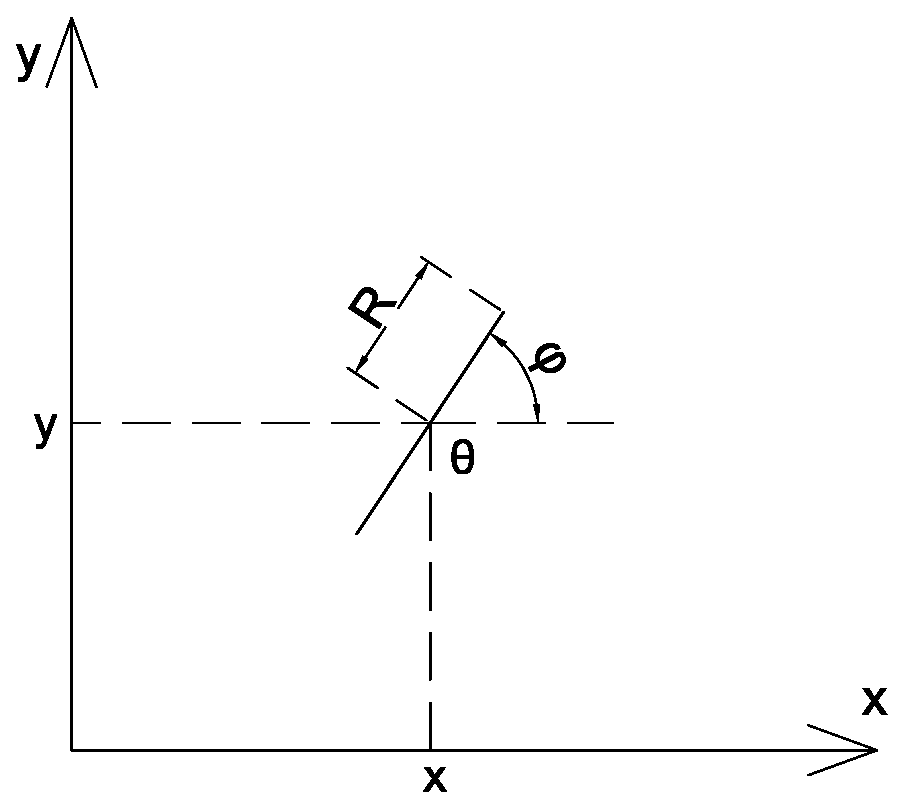
\includegraphics[width=0.5\textwidth]{img/uni.eps}
\caption{Unicycle}
\label{fig:uni_sch}
\end{figure}
In order to preserve dimensional consistency define the configuration vector in the following way:
$w = (x, y, \phi R, \theta R)^T$, where $R$ is the radius of the wheel.

The equation of motion can be presented
in the form $Q(w)\ddot w =F(w, \dot w)+Bu$. This can be easily acquired with usage of
Euler-Lagrange formalism. The inertia matrix is
$Q(w)=\mathrm{diag}\left\{m, m, \frac{I_\phi}{R^2}, \frac{I_\theta}{R^2}\right\}$ and
the input matrix is $B=\begin{bmatrix}
0_{2 \times 2} & I_2
\end{bmatrix}^T$, where $m$ denotes the wheel mass and $I_\phi=\frac{1}{4}mR^2$,
$I_\theta=\frac{1}{2}mR^2$.

When it comes to slips reaction forces, the Pfaffian matrix needs to be defined as
\begin{equation}
H(w)=\begin{bmatrix}
-\sin\phi & \cos\phi & 0 & 0\\
\cos\phi & \sin\phi & 0 & -1
\end{bmatrix}=\begin{bmatrix}
H^1(w)\\
H^2(w)
\end{bmatrix}.
\end{equation}
The constraints put in form $H(w)\dot{w}=0$ mean lack of lateral slip ($H^1(w)\dot{w}=0$) and lack of
longitudinal slip ($H^2(w)\dot{w}=0$).
The slips can be calculated as follows: the lateral slip $s_\perp=H^1(w)\dot w$ and the longitudinal slip $s_\parallel=H^2(w)\dot w$. With this quantities, the slip reaction forces may be defined as 
\begin{equation}
F(w, \dot w)=mg\epsilon s_\perp\frac{H^{1T}(w)}{||H^{1T}(w)||} + mg\tau s_\parallel\frac{H^{2T}(w)}{||H^{2T}(w)||},
\end{equation}
where $g$ is gravitational acceleration, $\epsilon$ and $\tau$ are lateral and longitudinal friction coefficients, respectively.

Transforming the system into a standard control form we finally obtain
\begin{equation}
\frac{\ud}{\ud t}\begin{pmatrix}
w \\ \dot w
\end{pmatrix}
 = 
 \begin{bmatrix}
 \dot w \\ Q^{-1}(w)F(w, \dot w)
 \end{bmatrix}+\begin{bmatrix}
 0_{4\times 2} \\ Q^{-1}(w)B
 \end{bmatrix}.
\end{equation}
\section{RobRex mobile manipulator}
The model consists of two parts: a mobile platform and a manipulator. The platform has got four
fixed-axis wheels, which are actuated with two motors --- the wheels on both sides are coupled.
The schematic structure of the vehicle is shown in figure \ref{fig:robrex_sch}
\begin{figure}
\centering
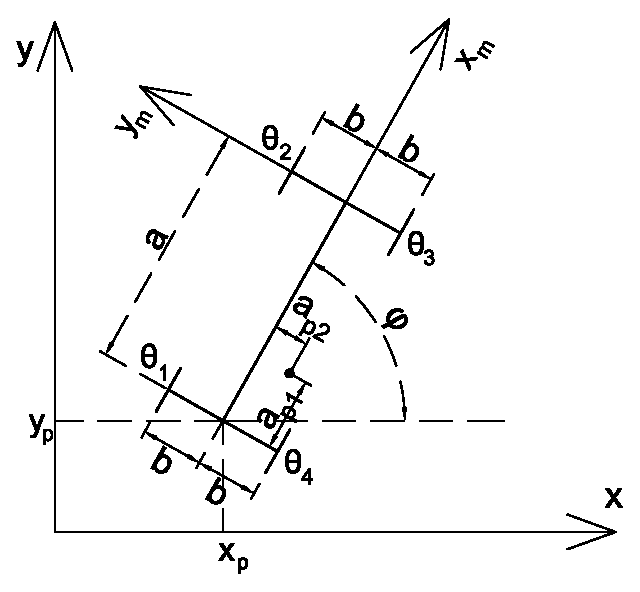
\includegraphics[width=0.7\textwidth]{img/robrex.eps}
\caption{Mobile platform Rex}
\label{fig:robrex_sch}
\end{figure}
The manipulator is mounted on the platform above the centre of the front wheel axis.
\subsection{Mobile platform}
Let $w\in \mathbb{R}^5$ be the configuration of the platform, where
$w=(x_p, y_p, a\phi, R\theta_{14}, R\theta_{23})$ and $\theta_1=\theta_4=\theta_{14}$, $\theta_2=\theta_3=\theta_{23}$.  
The dynamics model of the platform is represented in the standard form
\begin{equation}
\label{eq:std_mdl}
P(w)\ddot w + D(w, \dot w) = F(w, \dot w) + Bu.
\end{equation}
The elaborate model derivation can be found in \cite{coupled}. 
The elements of \eqref{eq:std_mdl} are equal to
\begin{align}
P(w) &= \begin{bmatrix}
Q_{11} & 0 & \frac{Q_{13}}{a} & 0 & 0\\
0 & Q_{22} & \frac{Q_{23}}{a} & 0 & 0\\
\frac{Q_{13}}{a} & \frac{Q_{23}}{a} & \frac{Q_{33}}{a} & 0 & 0\\
0 & 0 & 0 & \frac{Q_{44}}{R^2} & 0 \\
0 & 0 & 0 & 0 & \frac{Q_{55}}{R^2}
\end{bmatrix}, & 
D(w, \dot w) &= \frac{\dot w_3^2}{a^2}\begin{pmatrix}
-Q_{23} & Q_{13} & 0 & 0 & 0
\end{pmatrix}^T.
\end{align}
The components of the above equations are
\begin{align}
Q_{11} &= Q_{22} = m_p+4m_w, \phantom{xxxxxxxxxxx} Q_{44} = Q_{55} = 2I_{w33},\\
Q_{13} &= -m_p(a_{p1}\sin\frac{w_3}{a}+a_{p2}\cos\frac{w_3}{a})- 2m_wa\sin\frac{w_3}{a}, & &\\
Q_{23} &=  m_p(a_{p1}\cos\frac{w_3}{a}-a_{p2}\sin\frac{w_3}{a})+ 2m_wa\cos\frac{w_3}{a}, & &\\
Q_{33} &= I_{p33}+m_p(a_{p1}^2+a_{p2}^2)+4(I_{w11}+m_wb^2)+2m_wa^2.
\end{align}

The meaning of used symbols is:
\begin{itemize}
\item $a$ --- the distance between the front and the rear axis,
\item $m_p$ --- platform mass,
\item $m_w$ --- mass of one wheel,
\item $a_{p1}$, $a_{p2}$ --- coordinates of the platform's centre of mass with
respect to the platform's coordinate system,
\item $I_{w11}$ --- wheel's moment of inertia with respect to X axis,
\item $I_{w33}$ --- wheel's moment of inertia with respect to Z axis,
\item $I_{p33}$ --- platform's moment of inertia with respect to Z axis.

\end{itemize}

Motion constraints of the platform may be written in the Pfaffian form which is 
\begin{equation}
\label{eq:pfaff}
H(w)=\begin{bmatrix}
-\sin\frac{w_3}{a} & \cos\frac{w_3}{a} & 0 & 0 & 0\\
-\sin\frac{w_3}{a} & \cos\frac{w_3}{a} & 1 & 0 & 0\\
\phantom{-}\cos\frac{w_3}{a} & \sin\frac{w_3}{a} & -\frac{b}{a} & -1 & 0\\
 \phantom{-}\cos\frac{w_3}{a} & \sin\frac{w_3}{a} &  \frac{b}{a} &  0 & 1
\end{bmatrix} = \begin{bmatrix}
H^1(w)\\
H^2(w)\\
H^3(w)\\
H^4(w)
\end{bmatrix},
\end{equation}
where $H^1(w)$ corresponds to the lateral slip of rear wheels,
$H^2(w)$ to the lateral slip of front wheels,
$H^3(w)$ and $H^4(w)$ depict the longitudinal slips of the coupled left and right wheels, respectively.

Basing on the above matrix, the slips can be defined quantitatively in the following way
\begin{equation}
\begin{aligned}
s_{14} &= H_1(w)\dot w, & s_{12} &= H_3(w)\dot w,\\
s_{23} &= H_2(w)\dot w, & s_{34} &= H_4(w)\dot w,
\end{aligned}
\end{equation}
which leads to the slip reaction forces
\begin{equation}
\begin{aligned}
\label{eq:force_r}
R_{14}&=-(\epsilon_1 N_1 + \epsilon_4 N_4)s_{14}, & R_{12}&=-(\tau_1 N_1 + \tau_2 N_2)s_{12},\\
R_{23}&=-(\epsilon_2 N_2 + \epsilon_3 N_3)s_{23}, & R_{34}&=-(\tau_3 N_3 + \tau_4 N_4)s_{34},
\end{aligned}
\end{equation}
where $N_i$ are the normal forces applied by the wheels on the ground. We may assume that these
forces are equal to the quarter of the weight of the whole object: $N_i=\frac{m_p}{4}+m_w$ for $i=1, 2, 3, 4$.
Combining \eqref{eq:pfaff} and \eqref{eq:force_r}, we obtain
\begin{equation}
F(w, \dot{w}) = R_{14}\frac{H^{1T}(w)}{||H^{1T}(w)||} + R_{23}\frac{H^{2T}(w)}{||H^{2T}(w)||} + R_{12}\frac{H^{3T}(w)}{||H^{3T}(w)||} + R_{34}\frac{H^{4T}(w)}{||H^{4T}(w)||}.
\end{equation}
That means that the slips reaction forces are in the direction of transposed $H(w)$ matrix columns.

Due to the fact that the inputs are the torques applied to the both side coupled wheels,
the input matrix $B$ is equal to $\begin{bmatrix}
0_{2 \times 3} & I_2
\end{bmatrix}^T$ 

Reformulating the above into a standard control form leads to the following
\begin{equation}
\frac{\ud}{\ud t}\begin{pmatrix}
w \\ \dot w
\end{pmatrix}
 = 
 \begin{bmatrix}
 \dot w \\ P^{-1}(w)\left( F(w, \dot w) - D(w, \dot w) \right)
 \end{bmatrix}+\begin{bmatrix}
 0_{5\times 2} \\ P^{-1}(w)B
 \end{bmatrix}.
\end{equation}
\subsection{Manipulator arm}
\label{sec:manipul}
The manipulator has got five rotational joints. Its structure is shown in figure \ref{fig:manip}.
Let $x\in \mathbb{R}^5$ denote the configuration of the arm and $a_1, \dots, a_5$ the lengths of the links. The individual transformation matrices in the Denavit-Hartenberg convention are as follows:
\begin{equation}
\begin{aligned}
A_0^1(x_1) &= \rot(Z, x_1)\rot(X, \frac{\pi}{2}),\\
A_1^2(x_2) &= \rot(Z, x_2)\tr (X, a_2)\rot(X, -\frac{\pi}{2}),\\
A_2^3(x_3) &= \rot(Z, x_3)\tr (X, a_3)\rot(X, \frac{\pi}{2}),\\
A_3^4(x_4) &= \rot(Z, x_4)\tr (X, a_4)\rot(X, -\frac{\pi}{2}),\\
A_4^5(x_5) &= \rot(Z, x_5)\tr (X, a_5).
\end{aligned}
\end{equation}
In order to reduce the kinematics complexity and to facilitate obtaining the output function in the Euler angles form, it has been assumed that the rotation of joint 3 is fixed to $0$. This results in the transformation matrix $
A_0^5(x)=\begin{bmatrix}
R_0^5(x) & T_0^5(x)\\
0 & 1
\end{bmatrix}$, 
where
\begin{align}
T_0^5(x) &= \begin{pmatrix}
c_1\left((a_2+a_3)c_2 + c_{24}(a_4+a_5c_5)\right) - a_5s_1s_5\\
s_1\left((a_2+a_3)c_2 + c_{24}(a_4+a_5c_5)\right) + a_5c_1s_5\\
    (a_2+a_3)s_2 + s_{24}(a_4+a_5c_5)
\end{pmatrix},\\
R_0^5(x) &= \begin{bmatrix}
c_1c_{24}c_5-s_1s_5 & -s_1c_5-c_1c_{24}s_5 & -c_1s_{24}\\
s_1c_{24}c_5-c_1s_5 &  c_1c_5-s_1c_{24}s_5 & -s_1s_{24}\\
s_{24}c_5           & -s_{24}s_5           &  c_{24}
\end{bmatrix}.
\end{align}
The notation used in above formulae is: $s_i = \sin(x_i)$, $c_i=\cos(x_i)$, $s_{ij}=\sin(x_i+x_j)$,
$c_{ij}=\cos(x_i+c_j)$.
The end effector orientation Euler angles (using $\rot(Z,\phi)\rot(X, \theta)\rot(Z, \psi)$) are: $\phi=x_1-\frac{\pi}{2}$, $\theta=x_2+x_4$, $\psi=x_5+\frac{\pi}{2}$.
\begin{figure}[htb]
\centering
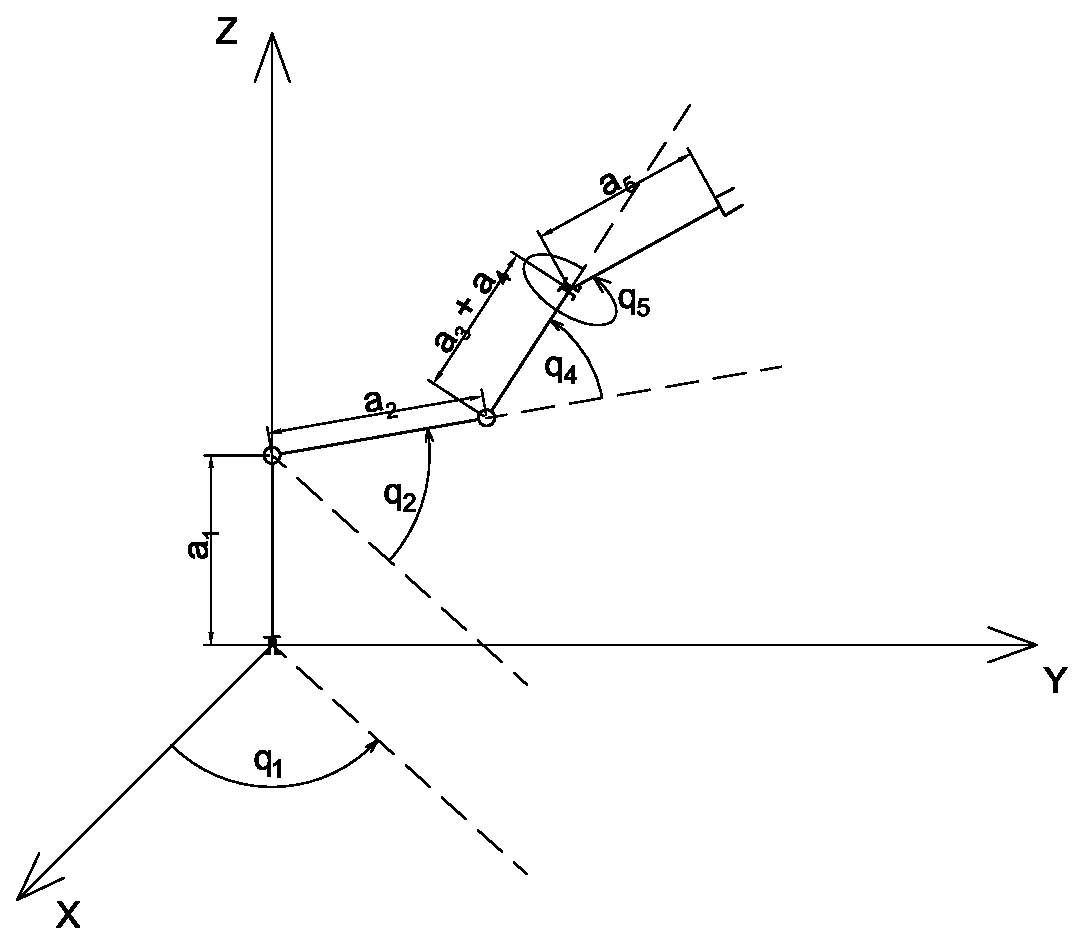
\includegraphics[width=0.7\textwidth]{img/manip.eps}
\caption{Manipulator structure}
\label{fig:manip}
\end{figure}
\paragraph{Global coordinate system}
In order to transform the manipulator's coordinate system into the global frame the transformation matrix needs to be calculated.
\begin{equation}
\begin{aligned}
A_m^g(w)&=\tr(X, w_1)\tr(Y, w_2)\rot\left(Z, \frac{w_3}{a}\right)\\
&= \begin{bmatrix}
\cos \frac{w_3}{a} & -\sin \frac{w_3}{a} & 0 & w_1+a\cos \frac{w_3}{a}\\
\sin \frac{w_3}{a} & \phantom{-}\cos \frac{w_3}{a} & 0 & w_2+a\sin \frac{w_3}{a}\\
0 & 0 & 1 & 0\\
0 & 0 & 0 & 1
\end{bmatrix}.
\end{aligned}
\end{equation}
In the global coordinate system the Euler angles are: $\phi=\frac{w_3}{a}+x_1-\frac{\pi}{2}$, $\theta=x_2+x_4$, $\psi=x_5+\frac{\pi}{2}$.
